\section{Opgave 1 - Binary circular watch}
\begin{enumerate}
	\item[1)]
	Vi skriver koden for vores cirkulære ur som det ses i kode \ref{lst:Watch}.\\
	\begin{lstlisting}[caption={VHDL code for binary circular watch},label={lst:Watch}]
	library ieee;
	use ieee.std_logic_1164.all;
	use ieee.numeric_std.all;
	
	entity watch is
	port( clk, speed, reset : in std_logic;
	mode : in std_logic_vector(1 downto 0);
	seg1 : out std_logic_vector(6 downto 0);
	cout : out std_logic);
	bin_val : out std_logic_vector(3 downto 0));
	end watch;
	
	architecture clock of watch is
	
	begin
	u2: entity work.counter port map(clk => clk_out, reset => reset, mode => mode, seg => seg1, cout => cout, bin_val => bin_val);
	
	
	process (reset, clk)
	variable clk_count : integer range 0 to 50000000;
	begin
	if reset = '0' then
	clk_count := 0;
	cout <= '0';
	elsif rising_edge(clk) then
	clk_count := clk_count + 1;
	cout <= '0';
	if speed = '1' then
	if clk_count >= 50000000 then
	cout <= '1';
	clk_count := 0;
	end if;
	elsif speed = '0' then
	if clk_count >= 25000 then
	cout <= '1';
	clk_count := 0;
	end if;
	end if;
	end if;
	
	end process;
	
	end clock;
	
	\end{lstlisting}
	
	Koden for vores counter er illustreret i kode \ref{lst:Counter}
	
		\begin{lstlisting}[caption={VHDL code for binary circular counter},label={lst:Counter}]
		library ieee;
		use ieee.std_logic_1164.all;
		use ieee.numeric_std.all;
		
		entity counter is
		port( clk, reset : in std_logic;
		mode : in std_logic_vector(1 downto 0);
		bin_val : out std_logic_vector(3 downto 0);
		cout : out std_logic;
		seg : out std_logic_vector(6 downto 0));	
		end counter;
		
		architecture circular of counter is
		signal bin_val_sig : std_logic_vector(3 downto 0);
		signal cout_sig : std_logic;
		begin
		
		u1: entity work.BCDdecoder port map(dcba => bin_val_sig, seg => seg);
		
		process (clk, reset, mode, bin_val_sig)
		
		begin
		if reset = '0' then
		bin_val_sig <= "0000";
		cout_sig <= '0';
		elsif rising_edge(clk) then
		if mode = "00" then
		if bin_val_sig = "1001" then 
		bin_val_sig <= "0000";
		cout_sig <= '1';
		else
		bin_val_sig <= std_logic_vector(unsigned(bin_val_sig)+1);
		cout_sig <= '0';
		end if;
		elsif mode = "01" then
		if bin_val_sig = "0101" then 
		bin_val_sig <= "0000";
		cout_sig <= '1';
		else
		bin_val_sig <= std_logic_vector(unsigned(bin_val_sig)+1);
		cout_sig <= '0';
		end if;
		else 
		if bin_val_sig = "0010" then 
		bin_val_sig <= "0000";
		cout_sig <= '1';
		else
		bin_val_sig <= std_logic_vector(unsigned(bin_val_sig)+1);
		cout_sig <= '0';
		end if;
		end if;
		
		end if;
		
		end process;
		bin_val <= bin_val_sig;
		cout <= cout_sig;
		end circular;
		
		\end{lstlisting}
		
		Vi har her anvendt endnu en VHDL-fil kaldet BCD-decoder, som vi i tidligere øvelser har anvendt til at decode vores værdier til visning på et 7-segment display.
		
		Da uret skal kunne tælle op for hvert 5. milisekund i speed-mode, skal counteren kun nå til 25000, som det ses i linje 34.
		
\item[2)] Vi tester vores watch på DE2-boardet. På følgende billeder kan forskellige værdier for 7-segment displayet 'hex0' ses:
		\begin{figure}[h]
			\centering
			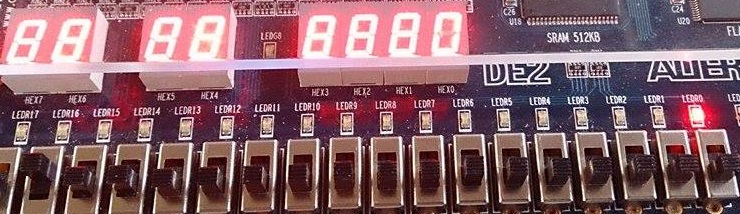
\includegraphics[scale=0.8]{pictures/Oevelse6/opg1/watch0.JPG}
			\caption{Uret er resat}
			\label{fig:alarm0}
		\end{figure}
		
		\begin{figure}[h]
			\centering
			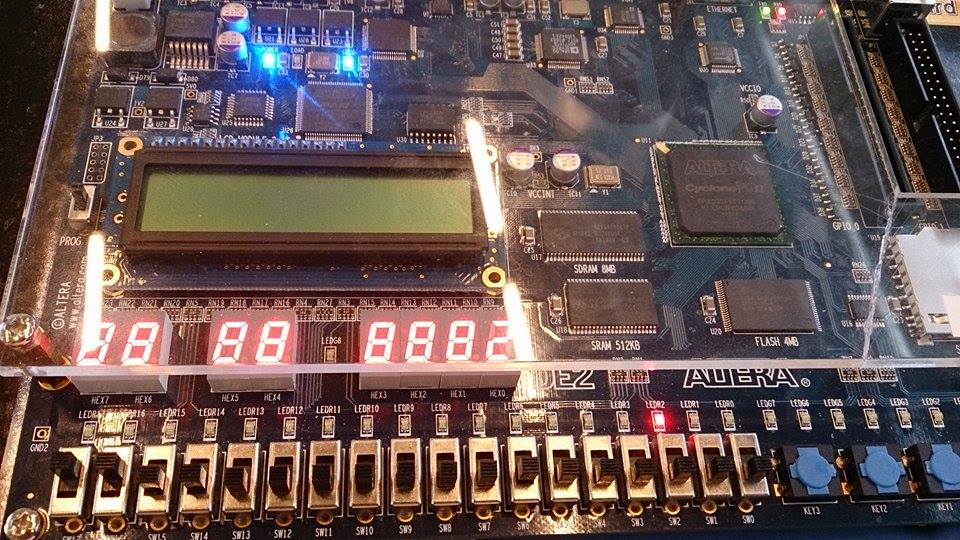
\includegraphics[scale=0.8]{pictures/Oevelse6/opg1/watch2.JPG}
			\caption{Uret viser 2}
			\label{fig:alarm2}
		\end{figure}

		\begin{figure}[h]
			\centering
			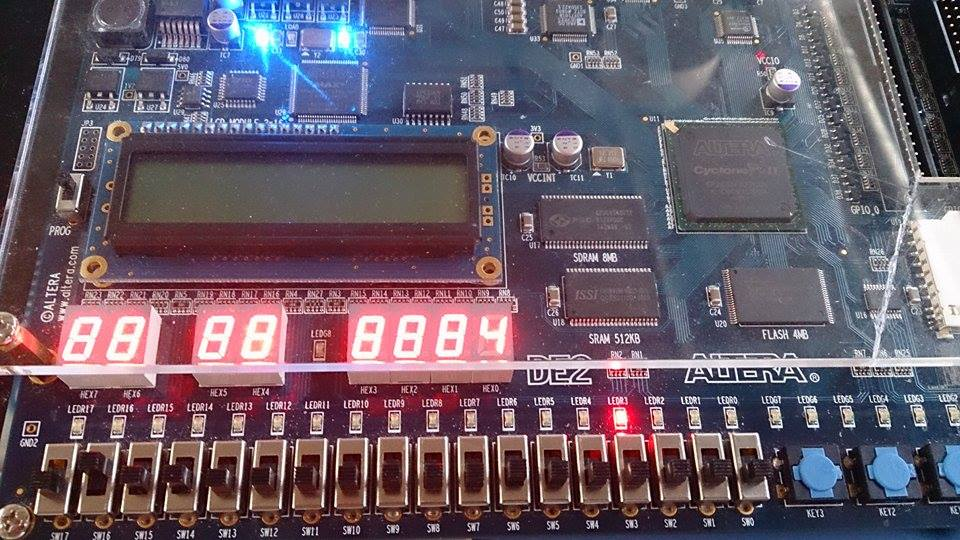
\includegraphics[scale=0.8]{pictures/Oevelse6/opg1/watch4.JPG}
			\caption{Uret viser 4}
			\label{fig:alarm4}
		\end{figure}


\end{enumerate}